%
% Cartoon showing the waves in the superseismic shock problem 
%
\begin{figure}[hbt]
\begin{center}
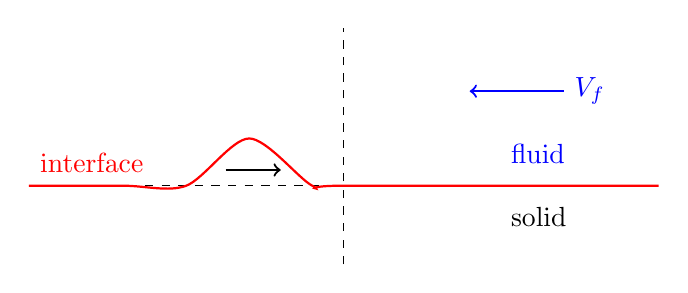
\begin{tikzpicture}[scale=4]
%- % axes: 
\draw[dashed] (-1.,0) -- (1.,0);
\draw[dashed] (0,-.25) -- (0,.5);
% -interface
\draw[thick,red] plot[smooth] coordinates {(-1,0) (-.7,0) (-0.5, 0) (-.3,.15) (-.1,0) (0.,0.) (1,0)};
% \draw[thick,red] plot[mark=x,smooth] coordinates {(-1,0) (-.3,0) (-.5,0) (-.3,.1 ) (-.1,0 ) (0,0) (.5,0) (1,0)}; 
%
\draw[thick,red] (-.8,.01) node[anchor=south] {interface};
\draw[blue] (.5, .1) node[anchor=west] {fluid}; 
\draw[black](.5,-.1) node[anchor=west] {solid};
%
\draw[->,thick,black] (-.375,.05) -- (-.2,.05);
\draw[<-,thick,blue] (.4,.3) -- (.7,.3) node[anchor=west] {$V_f$};
%- %
%- \draw[thick,blue] (0,0) -- (.3,.75) node[anchor=south] {shock wave};
%- \draw[blue] (.1,.5) node {$\xi$};
%- \draw[<->,thick,blue] (0,.4) arc (90:70:.4cm);
%- \draw[blue] (.4,.5) node {$\wv^0$};
%- \draw[blue] (-.4,.5) node {$\wv^1$};
%- % \draw[->,thick,blue] (.2,.63) -- (.4,.55); %  node[anchor=west]  {$V_s$};
%- %
%- \draw[blue] (.7, .2) node[anchor=west] {$V_f$}; 
%- %
%- \draw[thick,black,<-] (.5,-.2) -- (.7,-.2);
%- \draw[black](.7,-.2) node[anchor=west] {$V_s$}; 
%- \draw[black](.5,-.1) node[anchor=west] {solid};
%- % 
%- \draw[black] ( .2,-.5) node {$\overline{\wv}^0$};
%- \draw[black] (-.365,-.5) node {$\overline{\wv}^1$};
%- \draw[black] (-.8,-.4) node {$\overline{\wv}^2$};
%- %
%- \draw[thick,red] (0,0) -- ( 1.,0.);
%- \draw[red] (-.57,-.05) node {$\theta$};
%- \draw[<->,thick,red] (-.5,.0) arc (180:191:.5cm);
%- % 
%- \draw[thick,black] (0,0) -- ( -.25,-.75) node[anchor=north] {p-wave};
%- \draw[black] ( -.07,-.55) node {$\eta_p$};
%- \draw[<->,thick,black] (0,-.5) arc (270:252:.5cm);
%- % 
%- \draw[thick,black] (0,0) -- ( -.64,-.6) node[anchor=north] {s-wave};
%- \draw[black] (-.185,-.33) node {$\eta_s$};
%- \draw[<->,thick,black] (0,-.3) arc (270:225:.3cm);
\end{tikzpicture}
\end{center}
\caption{Problem configuration for an elastic Rayleigh wave in a compressible shear flow.}\label{fig:RayleighShearCartoon}
\end{figure}